
\documentclass[border=10pt]{standalone}
\usepackage{pgfplots}
\usepgfplotslibrary{fillbetween}
\pgfplotsset{compat=1.18}
\begin{document}
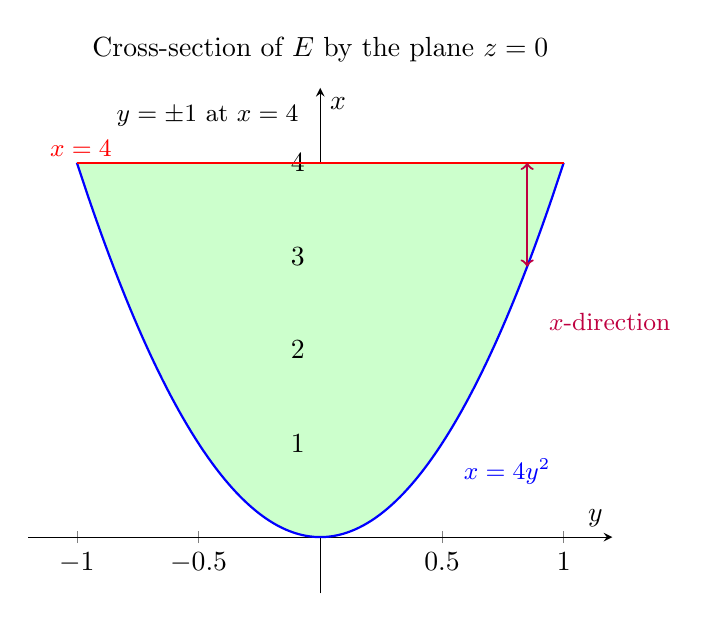
\begin{tikzpicture}
\begin{axis}[
    axis lines=middle,
    xlabel=$y$, ylabel=$x$,
    xmin=-1.2, xmax=1.2,
    ymin=-0.6, ymax=4.8,
    width=9cm, height=8cm,
    title={Cross-section of $E$ by the plane $z=0$},
    clip=false,
]
\addplot[blue, thick, domain=-1:1, samples=120, name path=A] ({x}, {4*x^2});
\addplot[red, thick, domain=-1:1, samples=2, name path=B] ({x}, {4});
\addplot[green!20] fill between[of=A and B];
\node[blue, font=\small, anchor=west] at (axis cs:0.55,0.7) {$x=4y^2$};
\node[red, font=\small, anchor=west] at (axis cs:-1.15,4.15) {$x=4$};
\draw[<->, purple, thick] (axis cs:0.85,4) -- (axis cs:0.85,{4*0.85^2});
\node[purple, font=\small, anchor=west] at (axis cs:0.9,2.3) {$x$-direction};
\node[font=\small, anchor=east] at (axis cs:-0.05,4.5) {$y=\pm1$ at $x=4$};
\end{axis}
\end{tikzpicture}
\end{document}
